The FPGA timetagger has a number of modular components. In this
section we will describe these pieces and how they fit together into
the larger system.

\begin{figure}
  \center
  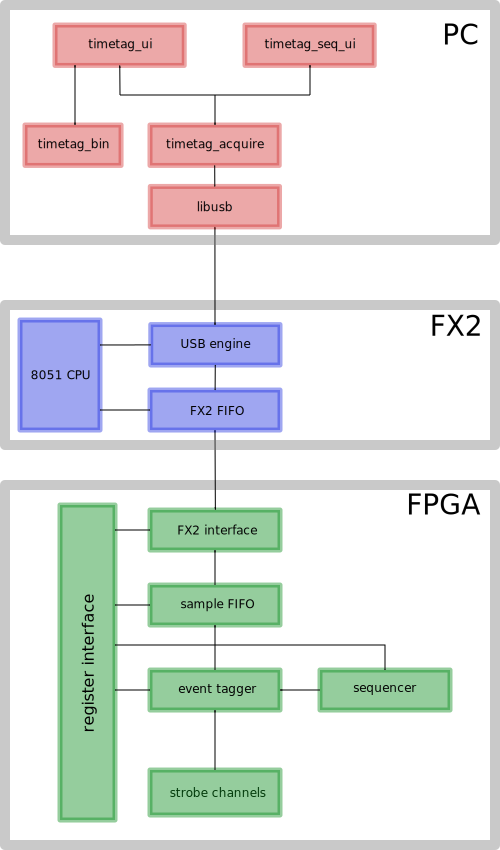
\includegraphics[scale=0.7]{block-diagram.pdf}
  \caption{A block diagram of the components of the timetagger.}
  \label{Fig:BlockDiagram}
\end{figure}

\section{FPGA implementation}
The core of the timetagger is implemented on the Xylo EM's Altera
EP2C5 FPGA. The logic is written in Verilog and can be found in the
{\tt timetag\_fpga} repository. As seen in FPGA block of
\ref{Fig:BlockDiagram}, the logic can be broken into a few functional
blocks,

\begin{itemize}
  \item event tagger: The core of the timetagger. Responsible for
    detecting events and producing timetagger records which are then
    queued in the sample FIFO
  \item sample FIFO: This is a buffer where event records wait until
    they can be sent to the FX2
  \item FX2 interface: This is a state machine which multiplexes
    access to the FX2 FIFO interface
  \item Register interface: This parses out commands from the host
    into register operations used to configure the various blocks of
    the device
\end{itemize}

Some of the discussion below will refer to details of the USB bus. The
interested reader is urged to read the Wikipedia article on this
subject and at very least the ``System Design''
section\footnote{\url{http://en.wikipedia.org/wiki/Usb#System_design}}.

\subsection{Record format}
The record format (found in {\tt timetag-fpga/docs/registers}) is reproduced below.

\verbatiminput{theory/timetag-fpga/docs/timetag-format}

\subsection{Register interface}
The register interface documentation (found in
{\tt timetag-fpga/docs/registers}) is reproduced below.

\verbatiminput{theory/timetag-fpga/docs/registers}

\subsection{Source files}
\begin{itemize}
  \item {\tt fx2\_timetag.v}: The top-level module of the design
  \begin{itemize}
    \item {\tt fx2\_bidir.v}: The FX2 interface state machine
    \item {\tt timetag.v}
    \begin{itemize}
      \item {\tt reg\_manager.v}: The register interface state machine
      \item {\tt readonly\_register.v}: Implementation of a read-only register
      \item {\tt sequencer.v}: The sequencer module
      \item {\tt apdtimer\_all.v}: The timetagger module
      \begin{itemize}
        \item {\tt event\_tagger.v}: The main timer and event tagger
        \item {\tt strobe\_latch.v}: The strobe trigger module
      \end{itemize}
      \item {\tt counter\_register.v}: A general counter exposed as a register
      \item {\tt sample\_fifo.v}: The sample FIFO
      \item {\tt sample\_multiplexer}: Convert 48 bit records to 8 byte records for the FIFO
    \end{itemize}
  \end{itemize}
\end{itemize}

\section{FX2 USB device}
The USB bus requires a complex protocol which would be difficult to
implement on an FPGA alone. For this reason, the Xylo EM board
includes a dedicated USB interface device, the Cypress FX2. This
device includes a USB engine, a few FIFOs to buffer data sent and
received from the bus, and a 8051 processor for high level
control. This microcontroller runs the firmware found in the
{\tt timetag\_fx2} repository. This firmware configures the device as
a simple USB passthrough as seen in \ref{Table:Endpoints}.

\begin{table}
  \begin{tabular}{|lll|}
    \hline
    Endpoint & Direction      & Purpose \\
    \hline
    EP2      & Host-to-Device & Commands from host to FPGA \\
    EP6      & Device-to-Host & Data from FPGA to host \\
    EP8      & Device-to-Host & Command replies from FPGA to host \\
    \hline
  \end{tabular}
  \caption{USB endpoint configuration}
  \label{Table:Endpoints}
\end{table}

The FX2 firmware has only a couple commands of its own as described in
{\tt timetag-fx2/README}. These are to adjust the queue depth (how
many records to queue up before sending a USB packet, exposed in
{\tt timetag\_ui} as the ``USB latency'').

\section{\tt timetag\_acquire}
{\tt timetag\_acquire} is a daemon which communicates with and
multiplexes access to the timetagger hardware. It is responsible for
abstracting the device's register interface and presents an ASCII
command interface through a UNIX domain socket
({\tt /tmp/timetag.sock}). One can interface directly with the daemon
with the {\tt netcat} utility,

\begin{verbatim}
$ nc -u /tmp/timetag.sock
\end{verbatim}

A description of the commands supported by this interface is available
with the {\tt help} command.

\section{\tt timetag\_ui}

{\tt timetag\_ui} is a Python GTK+ interface to the timetagging
functionality of the hardware. It communicates with {\tt
timetag\_acquire} through a UNIX domain socket and relies on several
of the other utilities in {\tt timetag\_tools} for low-level
processing of the incoming data stream (namely {\tt timetag\_bin}).

The capture backend (e.g. {\tt timetag\_acquire}) is somewhat
abstracted from the user interface and is handled by the {\tt
CapturePipeline} class.
In addition to the {\tt timetag\_acquire} backend, {\tt timetag\_ui}
accepts a {\tt --test} command-line option to use a test backend,
allowing testing of the frontend even in the absence of real
hardware. This test backend generates Poissonian emissions on each of
the enabled channels.

\section{\tt timetag\_seq\_ui}
{\tt timetag\_seq\_ui} is a Python GTK+ interface to the sequencer
functionality of the hardware. It communicates with
{\tt timetag\_acquire} through a UNIX domain socket.

